\section{Leseger"ate und -verfahren}
In diesem Kapitel sollen verschiedene Lesegeräte und ihre Anwendungsszenarien kurz vorgestellt werden.

\subsection{Handleser}
Bei den Handlesern gibt es verschiedene Funktionsweisen. Zum einen der \textbf{CCD-Handleser} für 1D-Codes. CCD steht für "Charged Coupled Device" (dt. \textit{ladungsgekoppeltes Bauteil}) und bezieht sich auf den eingebauten Sensor, der ein ebensolcher ist. CCD-Sensoren sind lichtempfindliche, elektronische Bauelemente, die auf dem inneren Photoeffekt beruhen\footnote{Zur näheren Funktionsweise des CCD-Sensors siehe zum Beispiel \url{http://www.ccd-sensor.de/}}. der CCD-Handleser ist im Prinzip aufgebaut wie eine Strichcode-Kamera mit CCD-Zeile. Da der Code mit ausreichend Kontrast auf dem Sensor abgebildet werden muss, muss er beleuchtet werden. Da eine Lichtquelle mit zunehmendem Abstand vom Sensor immer weniger Licht zur Umgebung hinzufügt, hat der CCD-Handleser einen Maximalabstand zum Code in Abhängigkeit zur Größe des Codes. Hinsichtlich der Neigung und Drehung ist der Handleser recht tolerant, sodass er auch bei einer Neigung von bis zu $\pm65^\circ$ zur Senkrechten und einer Drehung von bis zu $\pm80^\circ$ zur Senkrechten einen Barcode problemlos lesen kann (siehe dazu auch Abbildung~\ref{fig:neigungswinkel} und Abbildung~\ref{fig:drehwinkel}). CCD-Handleser werden mit integrierten Decodern gebaut und können über eine Vielzahl von Schnittstellen an bestehende Systeme angeschlossen werden, z.B. über USB, OCR, Tastaturemulation, \dots \\

\begin{figure}[htbp]
	\parbox{.47\textwidth}
	{
		\centering
		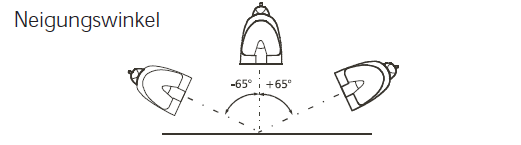
\includegraphics[height=2.5cm]{Bilder/Neigungswinkel.png}
		\caption[Neigungswinkel]{Neigungswinkel\footnotemark}
		\label{fig:neigungswinkel}
	}
	\hfill
	\parbox{.47\textwidth}
	{
		\centering
		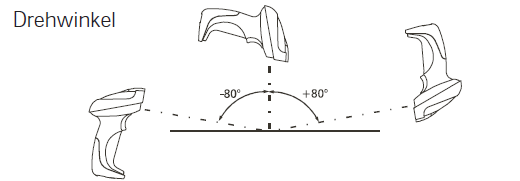
\includegraphics[height=2.5cm]{Bilder/Drehwinkel.png}
		\caption[Drehwinkel]{Drehwinkel\textsuperscript{\ref{ftn:first}}}
		\label{fig:drehwinkel}
	}
	\hfill
\end{figure}
\footnotetext{Quelle: \cite[64]{DatalogicScanning2007}\label{ftn:first}}


Ein weiterer Leser für 1D-Codes ist der \textbf{Handscanner auf Laserbasis}. Sein Leseprinzip ist von dem eines Laserscanners abgeleitet. Eingebaut ist in ihm eine Laserdiode, die einen Laserstrahl erzeugt, welcher über einen Schwingspiegel abgelenkt wird. Dadurch entsteht in der Leseebene ein wandernder Lichtfleck, der den Strichcode abtastet. Insgesamt erlaubt dieser Handscanner eine größere Distanz als der CCD-Handleser, jedoch ist er im Drehwinkel nicht ganz so tolerant (nur $\pm60^\circ$ zur Senkrechten). Er kann ebenfalls über eine Vielzahl von Schnittstellen an bestehende Systeme angebunden werden.

Der \textbf{2D-Leser} gehört zu einer neueren Generation von Barcodelesern und basiert intern auf Bildverarbeitungstechnologie. Das heißt, dass im Gerät eine kleine Kamera verbaut wurde, die ein Bild des Barcodes aufnimmt und dieses dann mithilfe integrierter Bildverarbeitungssoftware decodiert. Durch die Bildaufnahme ist der 2D-Leser in der Lage, alle gängigen eindimensionalen und zweidimensionalen Codes zu erfassen und zu verarbeiten. Die Kamera innerhalb des Geräts arbeitet wie der CCD-Handleser mit einem CCD-Sensor. Im Unterschied zum Handleser besteht die Kamera aber aus einem zweidimensionalen Sensor-Array (mehrere hundert Zeilen) und nicht nur aus einer CCD-Zeile. 
Die neueren 2D-Leser arbeiten allerdings nicht mehr mit CCD, sondern mit CMOS-Sensoren (\textit{\textbf{C}omplementary \textbf{M}etal \textbf{O}xide \textbf{S}emiconductor}\footnote{Näheres zu CMOS/CMOS-Sensoren findet man zum Beispiel unter \url{http://www.itwissen.info/definition/lexikon/complementary-symmetry-metal-oxide-semiconductor-CMOS-CMOS-Technologie.html} oder \url{http://www.itwissen.info/definition/lexikon/CMOS-Sensor-CMOS-sensor.html}}). Da diese Technik günstiger ist als die CCD-Technik, sind heute die meisten 2D-Leser auf dieser Basis aufgebaut. Auch sie können über verschiedene Schnittstellen an bestehende Systeme angeschlossen werden, zum Beispiel USB, Tastaturemulation oder aus Ethernet. Im Vergleich zu den 1D-Handlesern sind die 2D-Leser etwas eingeschränkter in ihrer Handhabung. Die Toleranz im Neigungswinkel liegt bei $\pm35^\circ$, die Toleranz im Drehwinkel bei $\pm40^\circ$, jeweils zur Senkrechten. Den 2D-Leser gibt es sowohl als Handscanner, als auch festmontiert zum Beispiel an einer Produktionsstraße oder einem Förderband \cite{DatalogicScanning2007}.   

\subsection{Funktionsweise der Laserscanner}
Innerhalb des Scanners (siehe Abbildung~\ref{fig:scannerschema} auf Seite~\pageref{fig:scannerschema}) erzeugt der Laser (1) einen für ihn üblichen, scharf gebündelten Lichtstrahl. Dieser trifft durch einen halb-durchlässigen oder durchbohrten Spiegel (5) auf ein sich drehendes, aus mehreren Spiegelelementen bestehendes Polygonrad (2). Durch dessen Drehung und die Reflexion an den Spiegelelementen wird der Laserstrahl durch das Austrittsfenster (4) immer in eine Ebene gelenkt.
In dieser Leseebene (im Bild zu sehen bei Nummer 3) entsteht nun ein wandernder Lichtpunkt. 
Befindet sich in der Leseebene ein Strichcode, so werden dessen Lücken und Striche von ebendiesem wandernden Lichtpunkt überstreift. Dabei reflektiert ein dunkler Strich durch seine schwarze Farbe ($\widehat{=}$ Absorption) weniger Licht als eine Lücke. Diese Unterschiede in der Reflexion werden im Lesegerät benutzt, um den Strichcode erst elektrisch und dann digital abzubilden. Ein Teil des reflektierten Lichts wird zurück in das Austrittsfenster geworfen und trifft wieder auf das Polygonrad. 
Von diesem wird es auf den Spiegel gelenkt, der das Licht auf eine Sammellinse (6) reflektiert, welche es bündelt und dadurch auf einen Fotodetektor (7) fokussiert.\pagebreak
In diesem Detektor werden nun die unterschiedlichen Intensitäten des auftreffenden Lichts in einen elektrischen Impuls umgewandelt. Dieser wird anschließend verstärkt und digitalisiert. Ein ebenfalls in dem Scanner vorhandener Decoder entschlüsselt nun die gemessenen Daten und leitet diese über die vorhandenen Schnittstellen an ein angeschlossenes System weiter. 
\begin{figure}[htbp]
	\centering
		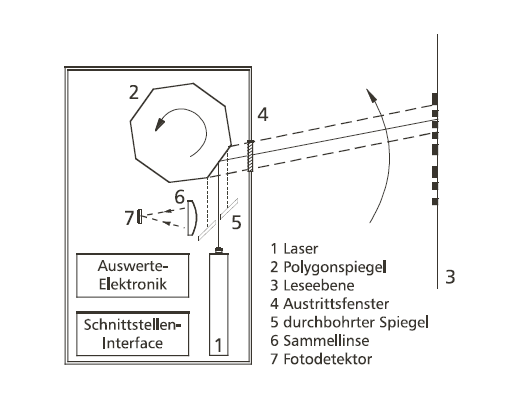
\includegraphics[width=10cm]{Bilder/Schema_Scanner.png}
		\caption[Schema eines Scanners]{Schema eines Scanners\footnotemark}
		\label{fig:scannerschema}
	\hfill
\end{figure}
\footnotetext{Quelle: \cite[67]{DatalogicScanning2007}}

\pagebreak
